\chapter{FAS系统具体设计内容}
\section{系统架构设计}
在设计FAS系统时,首先需要确立一个有效的系统架构。这个架构应该包括以下关键组成部分:

\begin{itemize}
	\item \textbf{中央控制室}:作为系统的核心,它负责实时监控所有火灾报警设备的状态,处理报警信号,并协调紧急响应。控制室应配备高级监控设备,如多屏幕显示系统和高效的通信设备,以确保在紧急情况下可以迅速做出反应。
	\item \textbf{分布式监控网络}:为了实现有效的监控和控制,需要在车站的各个关键区域部署传感器和报警设备。这些设备通过一个可靠的网络系统与中央控制室连接,以确保信息的实时传输。
	\item \textbf{数据管理和存储}:应设计一个数据管理系统来记录和分析火警事件和系统性能,以便于未来的优化和故障排查。
\end{itemize}

关键设备选型和布局

设计过程的下一个步骤是选择合适的设备,并确定其在车站中的布局。

\begin{itemize}
	\item \textbf{烟雾和热感应器}:这些是FAS系统中最重要的组成部分,它们需要被策略性地放置在车站的所有关键区域,如站台、候车室、商业区和服务设施等地方。选择这些传感器时,需要考虑它们的灵敏度、响应时间和误报率。
	\item \textbf{手动报警装置和火灾警报器}:这些装置应布置在人员易于接触的位置,如出入口、紧急出口和走廊。它们应该是高可见性的,并且易于操作。
	\item \textbf{消防设备布置}:喷淋系统、消防水泵和其他灭火设备应根据车站的具体布局和潜在的火灾风险来布置。例如,在电气设备丰富的区域,可能需要安装特殊的气体灭火系统。
\end{itemize}

系统功能和操作模式

最后,需要设计系统的功能和操作模式以满足实际的应用需求。

\begin{itemize}
	\item \textbf{自动监测和报警功能}:系统应能够自动监测火灾的迹象,如烟雾、热量或有害气体的增加,并及时激活警报。这包括自动启动喷淋系统和其他灭火设备。
	\item \textbf{手动控制和干预}:虽然系统主要是自动操作的,但也应提供手动控制选项,以便操作人员在特定情况下进行干预,如手动启动或关闭特定设备。
	\item \textbf{紧急响应和疏散指导}:在火灾发生时,系统应能引导乘客安全疏散,包括启动紧急照明和疏散指示牌,以及通过紧急广播系统发出指令。
\end{itemize}

火灾报警控制装置

火灾报警控制器是火灾自动报警系统的核心组件,扮演系统的指挥中心角色。其主要职责包括监视整个系统、报警管理、控制火警、显示信息、记录数据和存储档案等多重功能。\par 
在正常运行时,它会自动监视系统的状态并进行故障诊断,以及在出现火警情况时接收探测器和手动报警按钮的信号。随后,它会将这些信号转化为声音和光线的报警信号,同时标明报警的位置,并记录相关信息。此外,它还能启动自动灭火设备和消防联动控制装置,以应对火灾事件。\par 
火灾警报装置则是在火灾发生时通过声音、光线、语音等方式来提醒人们的消防设备。一些常见的装置包括警铃、警笛、声音报警器、光线报警器、声光报警器、语音报警器等。随着数字通信技术的进步,声音报警器和语音报警器的录音质量和保存能力有了显著提升,这使得警报的音响效果更具人性化,更容易引起人们的注意和反应。
\section{消防控制设备}
消防控制设备是用于协调和控制气体灭火设备、水消防设备、防排烟设备、防火卷帘门等各类消防设施的装置,以实现由火灾报警系统(FAS)直接或间接监测和管理消防设备及相关非消防设备的控制和切换。\\
这些设备主要包括以下部分:
\begin{itemize}
	\item 功能模块:用于实现特定控制和联动功能的模块,通常集成在消防控制设备中,以确保各种消防设备的协同工作。
	\item 消防联动控制柜:这是一个关键的组件,用于协调各种消防设施的操作,以应对火灾事件。它可以自动触发或关闭消防设备,确保火灾得到迅速的响应。
	\item 手动联动控制柜:这个设施通常位于火灾警报系统中,用于手动启动重要的消防设备。这是一个备用的手动控制系统,以确保在需要时可以手动干预消防设备的操作。
\end{itemize}
这些消防控制设备的目标是确保火灾报警系统能够有效地管理和控制各种消防设备,以最大程度地减少火灾的风险和损害。
\begin{figure}[!h]
	\centering
	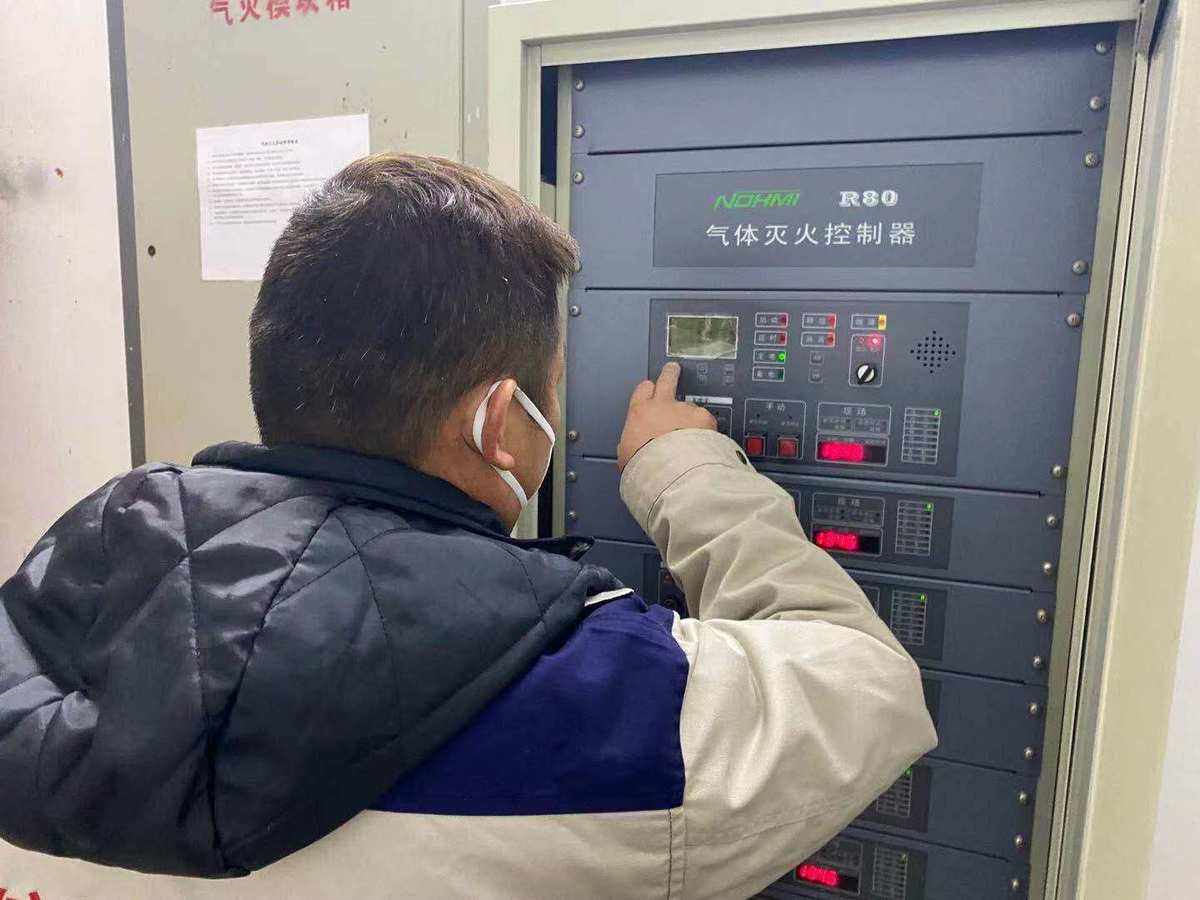
\includegraphics[width=0.5\textwidth]{地铁消防控制装置.png}
	\caption{地铁消防控制装置}
\end{figure}

传感器设备选型

在这个设计中,针对综合监控系统中的FAS系统,只配置车站级FAS系统中的传感器。每个监控对象都需要安装传感器来进行监测和测量。这些传感器用于检测各种空气参数,包括室内、室外和风管式的温度和湿度传感器,以及二氧化碳浓度传感器。此外,还需要用于空调水系统的压力、压差传感器、变送器、电磁流量计、水管式温度计和感温元件,通常使用PT100或PT100热电阻,并通过变送器将其转换为标准的0$\sim$10V信号,然后通过I/O接口连接到FAS系统。\par 
在这个设计中,采用了Honeywell公司提供的传感器。这些传感器的种类包括温度传感器、MEMS压力传感器、二氧化碳传感器、湿度传感器、灰尘传感器、NTC热敏电阻器、PTC热敏电阻器、表面贴装压力传感器、低压和中压传感器、高压传感器、一次性医用压力传感器、固态低中压传感器、中压传感器、过滤空气阻力(FAR)传感器、微型二氧化碳传感器、二氧化碳传感器模块、以及适用于恶劣环境的传感器等。\par 
这些传感器的选择和配置有助于确保FAS系统能够高效地监测和管理各种参数,以确保综合监控系统的正常运行和安全性。\par
温度传感器测量范围:\par 
\begin{enumerate}
	\item 室外:-40-60℃
	\item 室内:-10-50℃
	\item 水管道:0-60℃
	\item 风管道:-20-60℃
\end{enumerate}
\par 
湿度传感器测量范围:
\begin{enumerate}
	\item 室外、室内、风管道:0-99\%
\end{enumerate}
温湿度传感器的安装要求如下:\par 
风管及室外式温湿度传感器:这些传感器将被安装在通风风管、结构风道以及地下区间。温度传感器的阻值特性需要符合Pt1000级,遵循DIN60751标准,精度不低于±0.2℃(在20℃时);湿度传感器为电容式,精度不低于2\%。传感器的输出将是标准的电流或电压信号。其外壳可以是金属或塑料(需符合UL94-V0阻燃等级要求),端子盒的防护等级应达到IP65,同时需要配置施工安装所需的连接件。\par
室内式温湿度传感器:这些传感器将被安装在公共区域和设备房间内。温度传感器的阻值特性需要符合Pt1000级,遵循DIN60751标准,精度不低于±0.2℃(在23℃时);湿度传感器为电容式,精度不低于2\%。传感器的输出将是标准的电流或电压信号。其外壳可以是金属或塑料(需符合UL94-V0阻燃等级要求),防护等级应达到IP55,同时需要配置施工安装所需的连接件。\par 
这些传感器的精确性和耐用性是确保系统正常运行的关键因素,因此其制造和安装需要满足特定标准和要求。
% Please add the following required packages to your document preamble:
% \usepackage{multirow}
\begin{table}[h]
	\centering
	\caption{传感器数量}
	\renewcommand\arraystretch{2}
	\label{tab:传感器数量}
	\begin{tabular}{|c|c|c|c|c|}
		\hline
		\multirow{10}{*}{\textbf{传感器}} & 温度传感器     & 室外型 & 套 & \textbf{1}  \\ \cline{2-5} 
		& 湿度传感器     & 室外型 & 套 & \textbf{1}  \\ \cline{2-5} 
		& 温度传感器     & 水管型 & 套 & \textbf{2}  \\ \cline{2-5} 
		& 温度传感器     & 风管型 & 套 & \textbf{4}  \\ \cline{2-5} 
		& 湿度传感器     & 风管型 & 套 & \textbf{4}  \\ \cline{2-5} 
		& 温度传感器     & 室内型 & 套 & \textbf{10} \\ \cline{2-5} 
		& 湿度传感器     & 室内型 & 套 & \textbf{10} \\ \cline{2-5} 
		& 二氧化碳浓度传感器 & 室内型 & 套 & \textbf{3}  \\ \cline{2-5} 
		& 空调水流量传感器  & 水管型 & 套 & \textbf{1}  \\ \cline{2-5} 
		& 空调压力传感器   & 水管型 & 套 & \textbf{1}  \\ \hline
	\end{tabular}
\end{table}

地铁FAS的组成

地铁火灾报警系统主要由设置在各地铁车站、区间隧道、控制中心大楼、车辆段、停车场、主变电站等与地铁运营有关建筑与设施的火灾报警系统设备以及相关的网络设备和通信接口组成。系统分为三个级别:
\begin{enumerate}
	\item 设置在OCC的中央监控管理级。
	\item 车站(车站与车辆段)监控管理级。
	\item 现场控制级。
\end{enumerate}

中央监控管理级

中央监控管理级位于地铁控制中心,作为地铁消防的指挥和控制中心,其主要任务是监视地铁系统各个区域,包括车站、区间隧道、控制中心大楼、车辆段、停车场、主变电站等,以便实时检测火灾报警、消防联动以及故障情况。

在中央监控管理级,通常配置了防灾报警主机和FAS(Fire Alarm System)操作员工作站。FAS主机通常通过专用网络连接到整个系统的FAS专网,并与各防灾报警分机进行通信。此外,中央监控管理级的操作站也需要配置打印机等外围设备,以便记录和输出相关信息。

一般情况下,中央监控管理级的操作站上会设置FAS大屏幕或模拟显示屏,以图形的方式直观地显示全线各区域的火灾报警和故障信息。这样的可视化展示有助于支持全线的防灾和救灾指挥工作,使操作员能够更好地掌握和应对各种突发情况。

车站监控管理级和现场控制级

车站监控管理级和现场控制级由以下组成:车站FAS分机(火灾报警控制器)、车站FAS操作员工作站、打印机、消防联动控制柜以及现场的火灾探测器、控制和监视模块等设备。

车站控制室设置了FAS分机,也称为火灾报警控制器,它通过总线与现场设备相连,形成车站的火灾报警系统。这个设备负责处理车站内的火灾报警情况以及联动控制。此外,它通过FAS网络与其他车站的报警控制器和控制中心操作工作站进行通信,用于报告火灾报警、系统故障、联动控制以及各消防设备的运行状态等信息。

在车站控制室还设置了消防联动控制柜,该设备用于直接手动控制消防工况下运行的设备,例如消防泵、TVF分机、UPE/OTE风机、组合式空调箱、变风量主运调器、回二氧化碳检测机(同时也用于排烟风机)、小系统回风机、送风机等。这个控制柜通过硬连线的方式与所控制的消防设备的控制回路直接相连,以确保在火灾或其他紧急情况下能够手动控制这些设备的运行。

\begin{figure}[h]
	\centering
	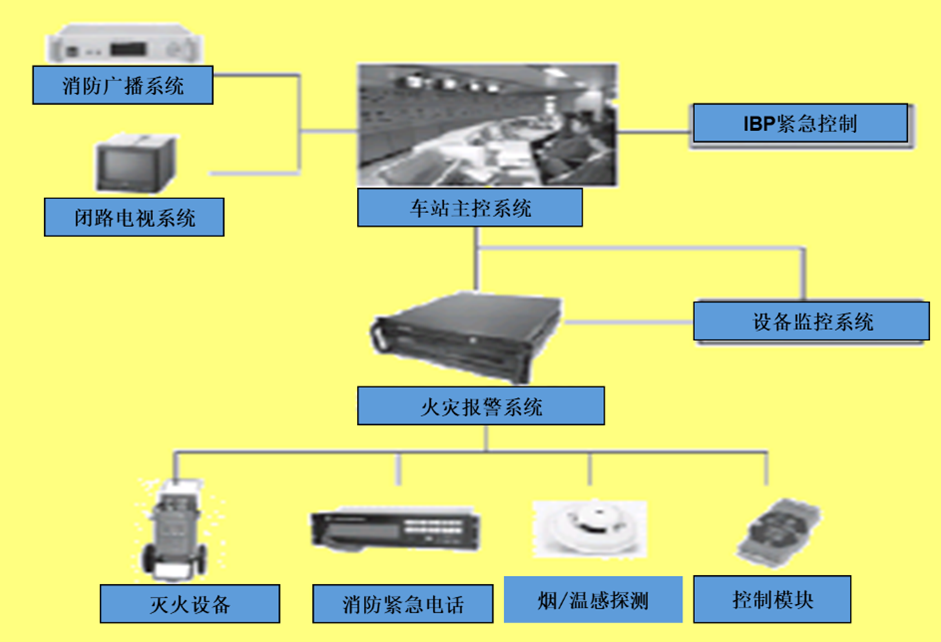
\includegraphics[width=0.8\textwidth]{FAS系统部署示意图.png}
	\label{FAS系统部署示意图}
	\caption{FAS系统部署示意图}
\end{figure}

\section{FAS专网接口设计}

中央监控管理级的操作工作站与车站监控管理级的火灾报警控制器之间通过FAS专用网络接口组成FAS系统独立的外网。由于火灾报警控制器与中央操作工作站直接通信,不受其他系统网络负荷和设备故障的影响,此网络通信方式响应速度较快,安全可靠。 

\begin{figure}[h]
	\centering
	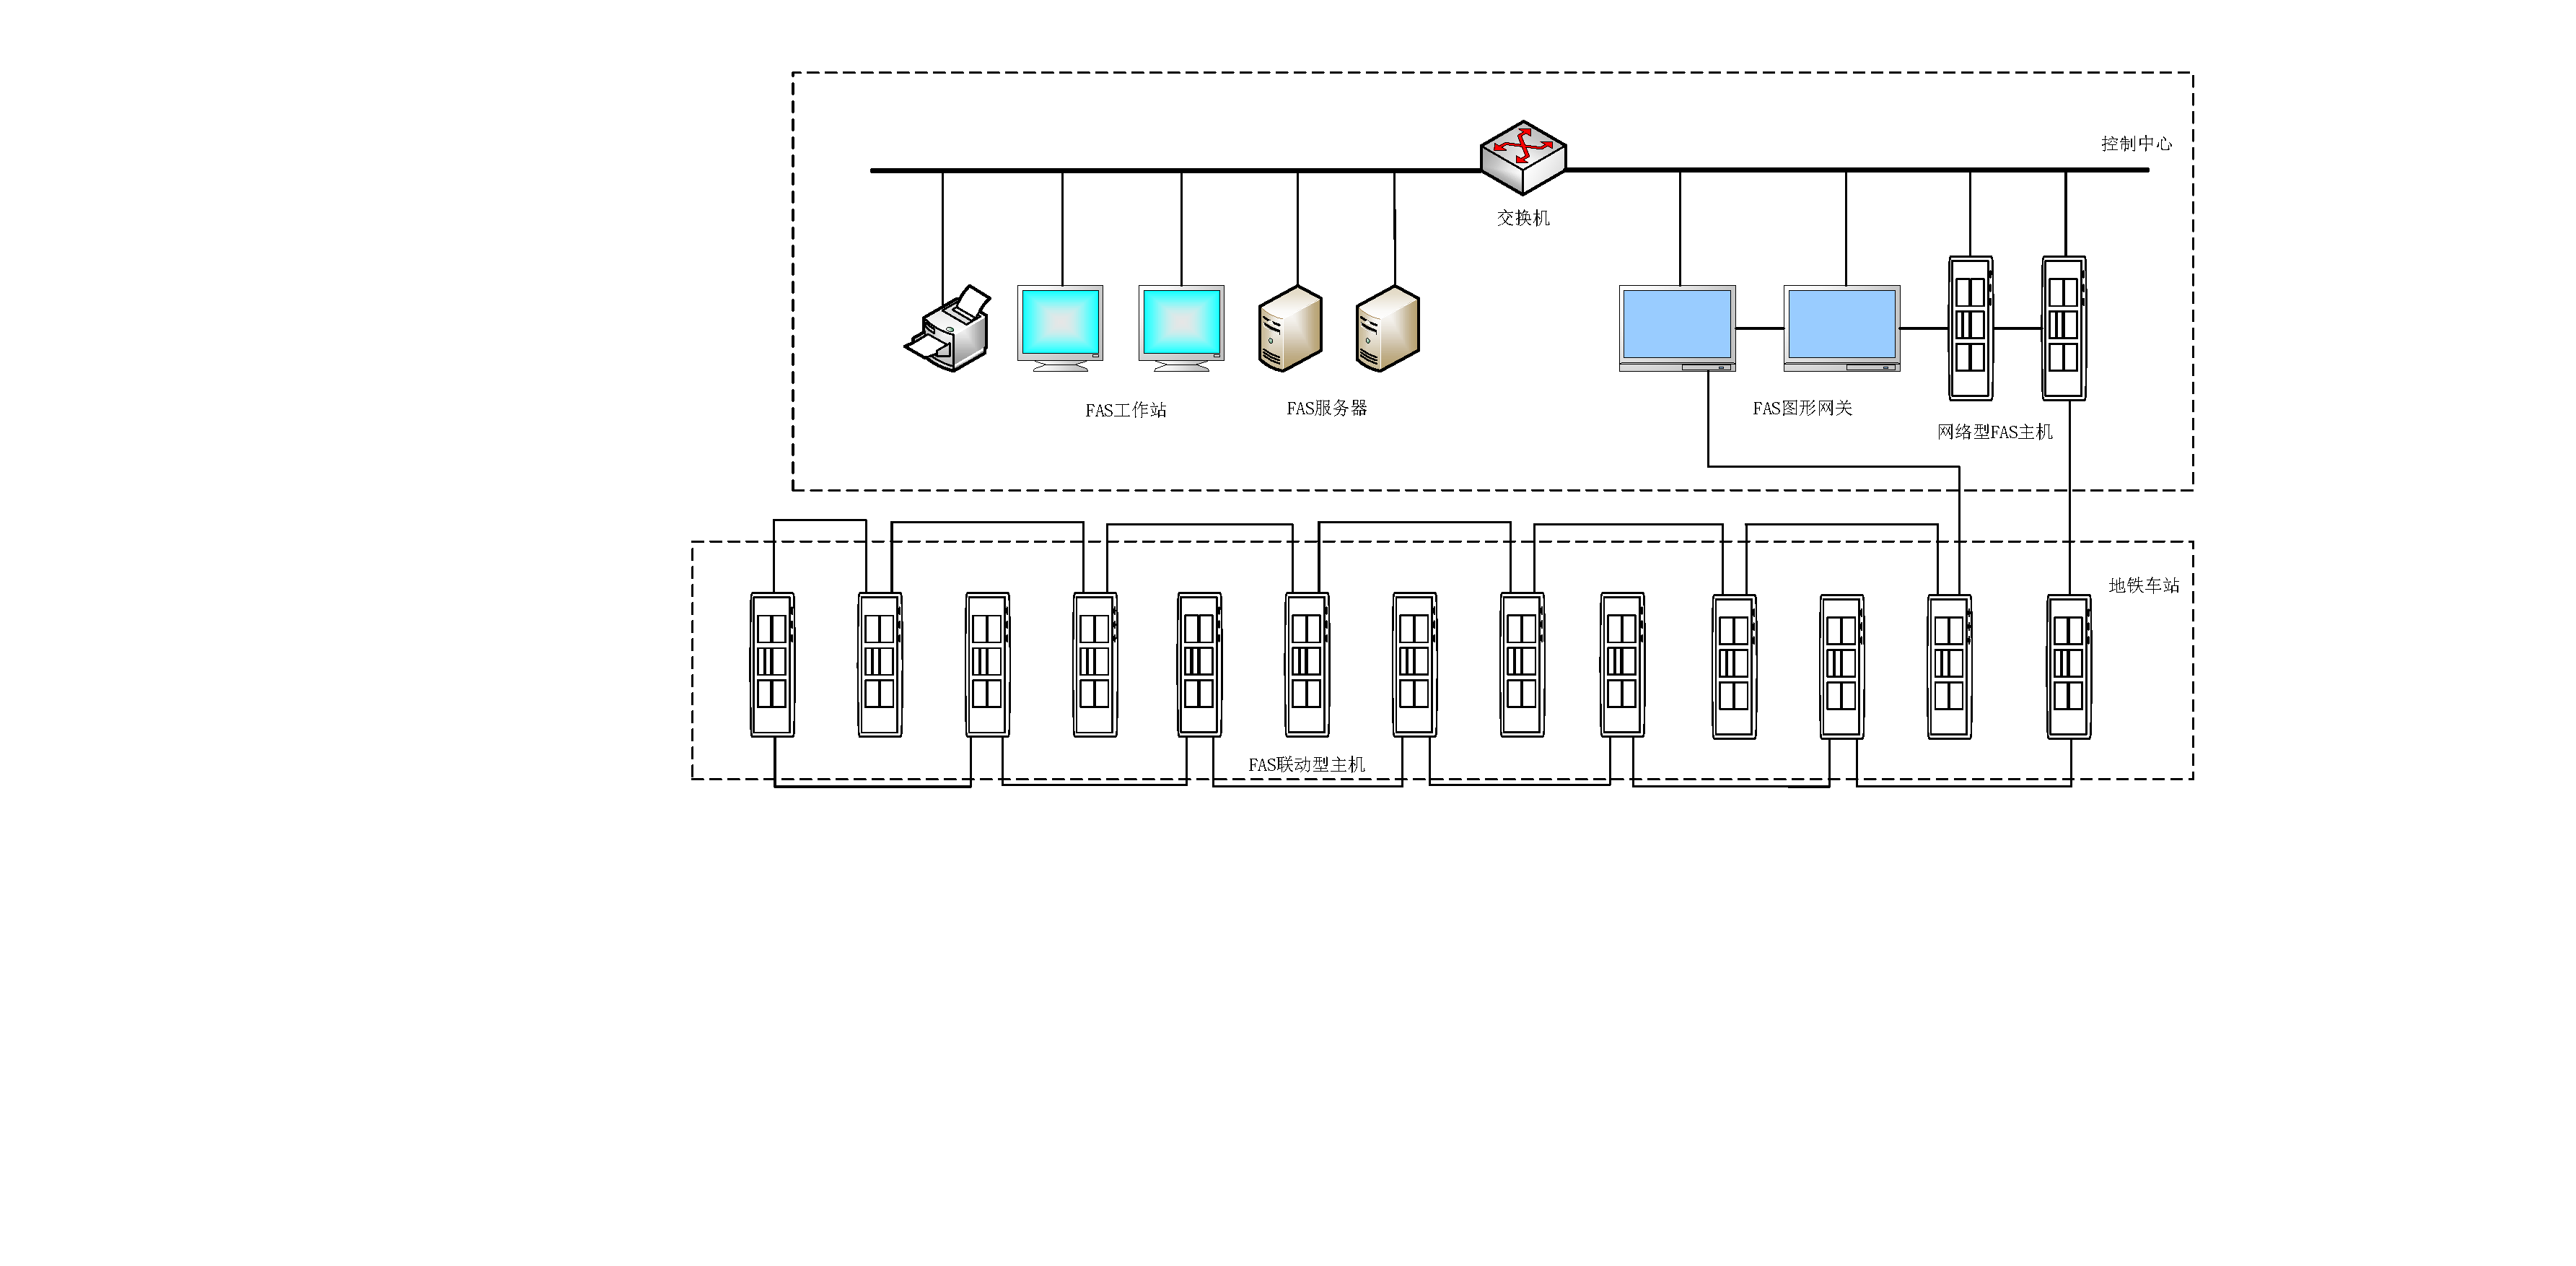
\includegraphics[width=0.8\textwidth]{FAS的网络拓扑结构.pdf}
	\label{FAS的网络拓扑结构}
	\caption{FAS的网络拓扑结构}
\end{figure}

地铁防灾报警系统的功能也分为中央级功能和车站级功能。
\begin{enumerate}
	\item 通过火灾报警网络接收并存储全线消防设备运行状态信息,远程监视就地消防设备的运行状态。主机通过显示画面和数据表格提供现场的监视信息,具有丰富的HMI画面,展现FAS的中央功能。
	\item 接收全线车站、车辆段、主变电站、指挥中心的火灾报警信息并显示报警部位。
	\item 控制中心声光报警系统发出声、光火灾警报信号。
	\item 打印机实时打印出火灾报警系统发生的时间、地点、火灾类等。
	\item 通过控制中心的网络向EMCS发出火灾紧急信息,并指令EMCS进入火灾报警处理模式。
	\item 通过闭路电视系统切换装置和显示终端确认火灾情况。当确认火灾发生后,在一定时间内如果现场火灾报警控制器还未做出反应,可在控制中心发出指令给站点火灾报警器,指挥现场的火灾抢救工作。
	\item 存储记录的功能:存储事件、记录和操作人员的各项操作记录。包括火警监视、故障状态、设各维修、清洗等信息记录。
	\item 系统编辑功能。在线编辑功能:具有相当权限的维护人员通过工作站能添加系统设备或直接在现场编辑,自定义设备。通过系统提供的程序监控软件,在防灾报警主机上进行在线编辑并输出至打印机或磁盘等。离线编辑功能:现场设备的定义和参数修改可在办公室的PC上完成,经编译转换后,到现场通过电话线(下载)将程序发送到火灾报警控制机上。 
	\item 历史档案管理:将报警、事件等信息记录归档处理。操作人员可根据要求随时进行信息的查看和打印输出。
\end{enumerate}

除以上功能外,FAS中央总站必须与其他子系统协调配合。
\begin{enumerate}
	\item 与有线、无线电话系统的协调。
	\begin{enumerate}
		\item 防灾指挥中心设置了与市消防、防汛、地震预报中心等部门联系的专用外部电话。
		\item 防灾指挥中心设置与车站设备系统共用的调度电话总机,各车站(车辆段、场、主变电所)等设置调度分机。
		\item 防灾指挥中心、各车站设置与列车司机联系的无线电话.
	\end{enumerate}
	\item 与广播系统配合:FAS系统不单独设置消防广播、与公共广播系统合用。
	\item 闭路电视监视系统
\end{enumerate}

FAS系统与行车管理等共用一套闭路电视系统,在防灾指挥中心设置切换装置和显示终端。当地铁发生灾害时,切换为防灾监视

\section{FAS的接口}
\subsection{与气体灭火系统的接口}
如果地铁工程的气体灭火控制系统采用探、控、火为一体的方案,则FAS与灭火的接口非常简单便捷,只需通过系统内部网卡接口即可。这种同一系统的内部连接,最大限度保证了地铁工程消防系统完整性、安全性,并可节约投资,同时,也利于系统将来的维护管理。

如果灭火系统与FAS是不同的两个系统,则需要系统间就接口问题进行协商,此时以FAS系统供货商为主。

根据国标,BAS系统已经承担了多项消防联动控制功能,并具备了标准中规定的有关控制方式、响应性、反馈显示等技术要求。因此BAS和FAS之间有着紧密的联系,特别是在火灾工况下,两个系统需要共同完成消防联动控制。BAS需要通过通信方式和FAS主机进行接口,通过该接口接收FAS确认的火灾报警信息,用来触发模式控制。如\ref{BAS系统与FAS系统接口图}所示:

\begin{figure}[h]
	\centering
	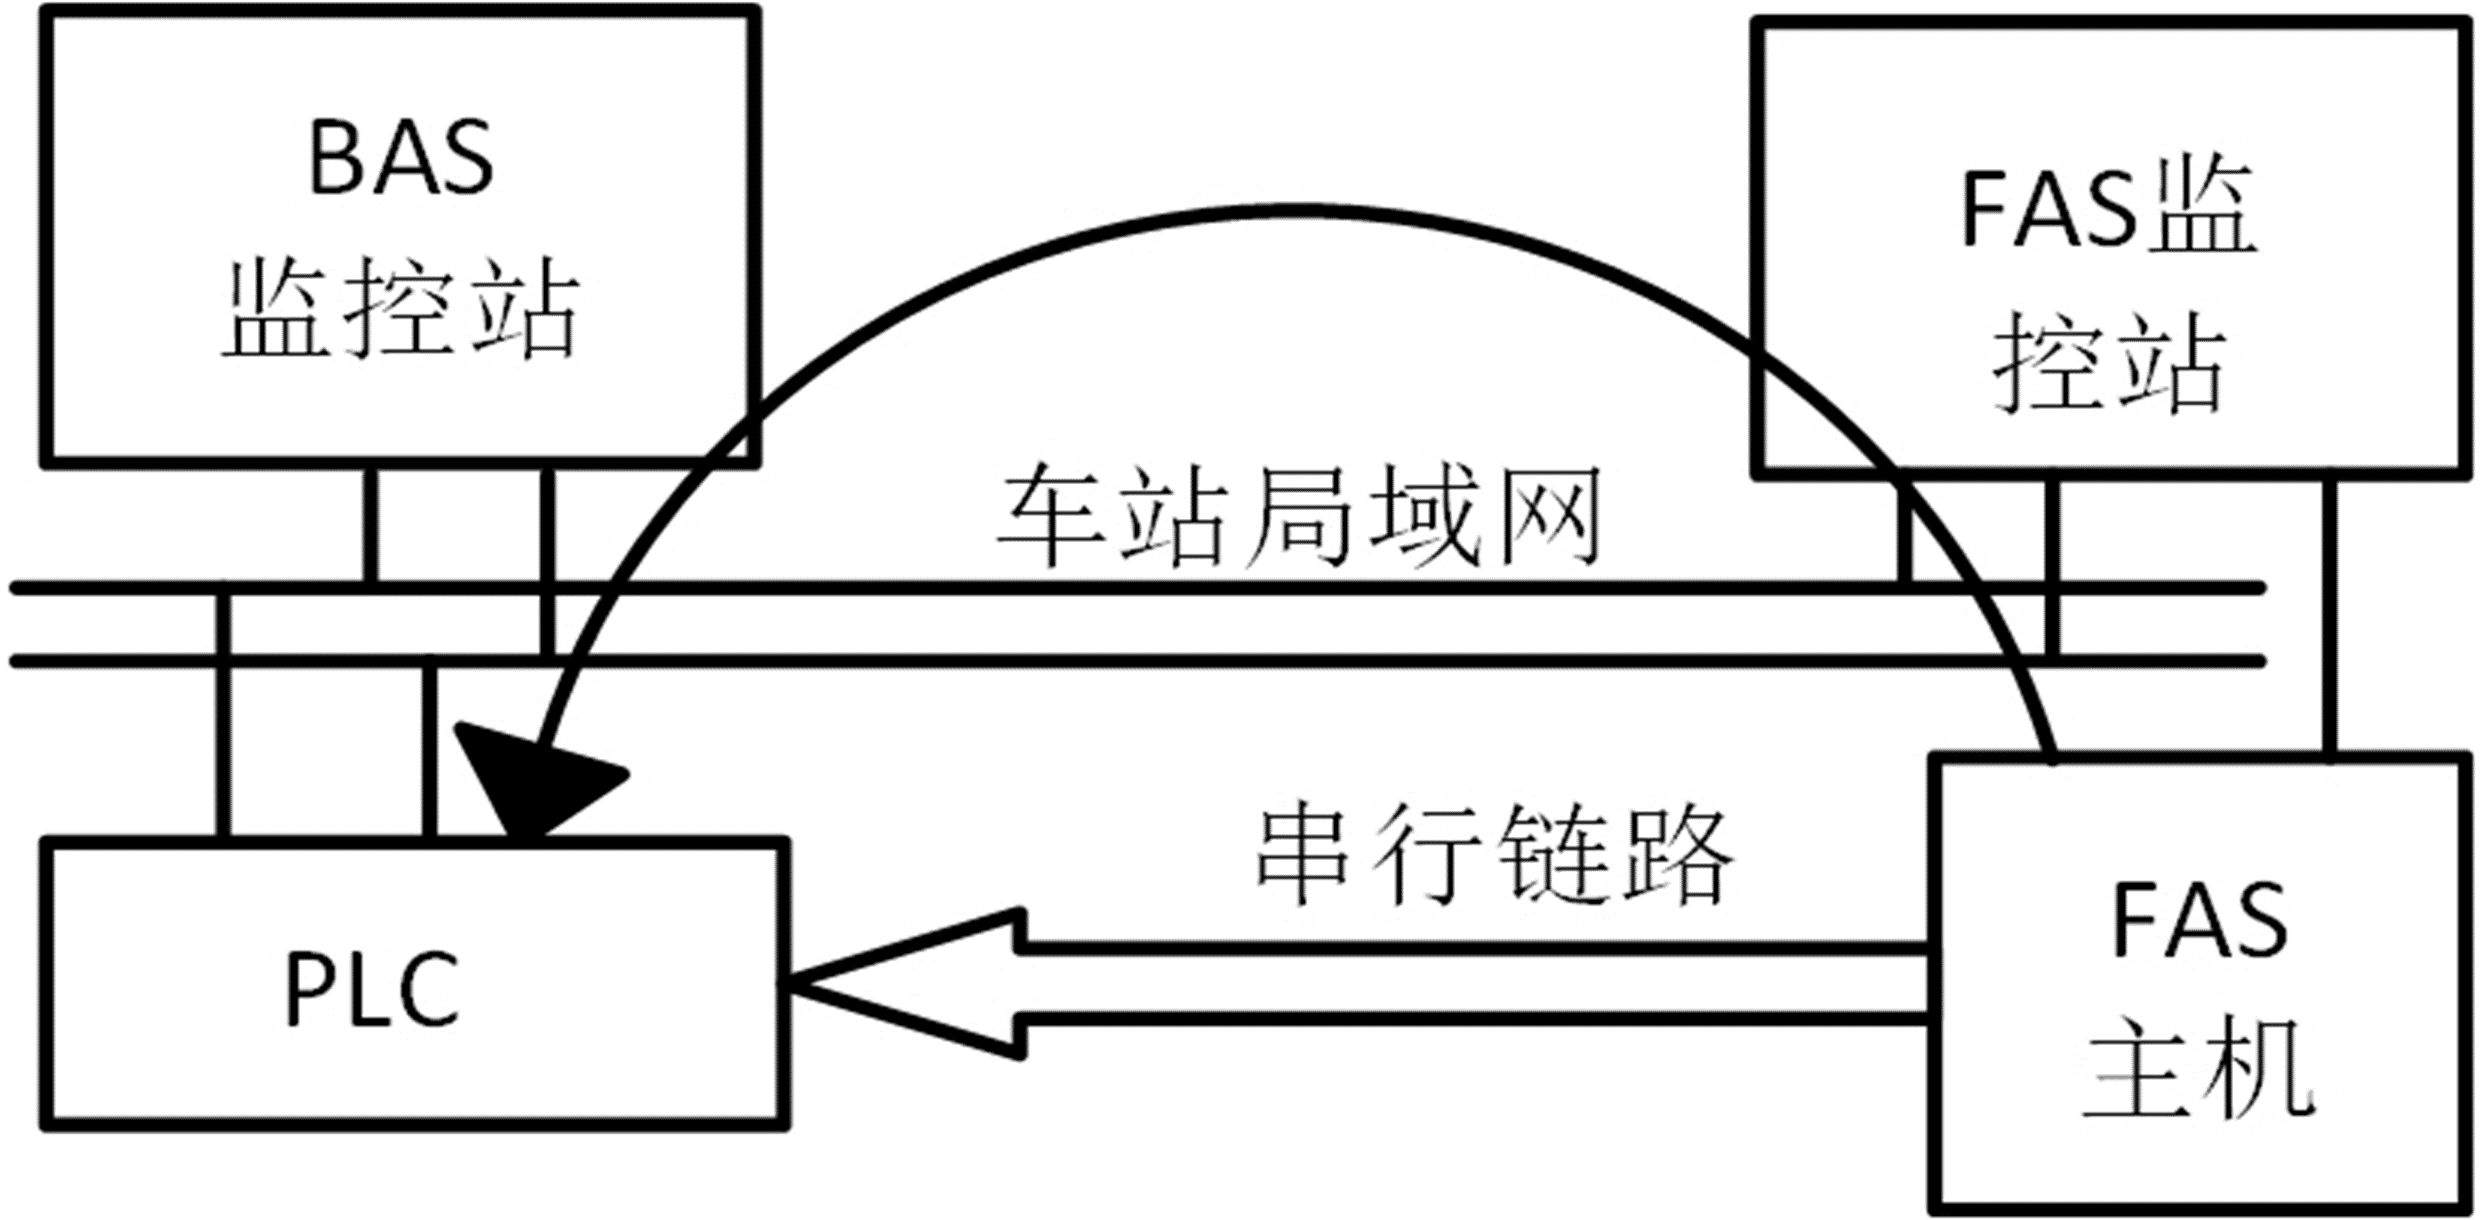
\includegraphics[width=0.8\textwidth]{BAS系统与FAS系统接口图.png}
	\caption{BAS系统与FAS系统接口图}
	\label{BAS系统与FAS系统接口图}
\end{figure}

\subsection{与EMCS系统的接口}
FAS系统和EMCS系统在主控级和分控级均设有数据传输接口,接口界面在防灾报警主机和防灾报警分机上。

防灾报警系统发出的指令应具有最高优先权,当发生火灾时,通过车站的数据接口发出救灾指令给EMCS系统, EMCS将其所监控的设备运行状态转换为预定的火灾运行模式。

主控级采用网络连网方式提供数据接口。 FAS系统主控制计算机作为整个地铁调度管理网络的一个节点,通过骨干网连接车站监控网实现与EMCS的控制主机交换的数据接口。

当FAS系统发出火灾报警信号时, FAS主机直接向网络发出火灾指令,并使FAS强制进入火灾运行模式。

\begin{figure}[h]
	\centering
	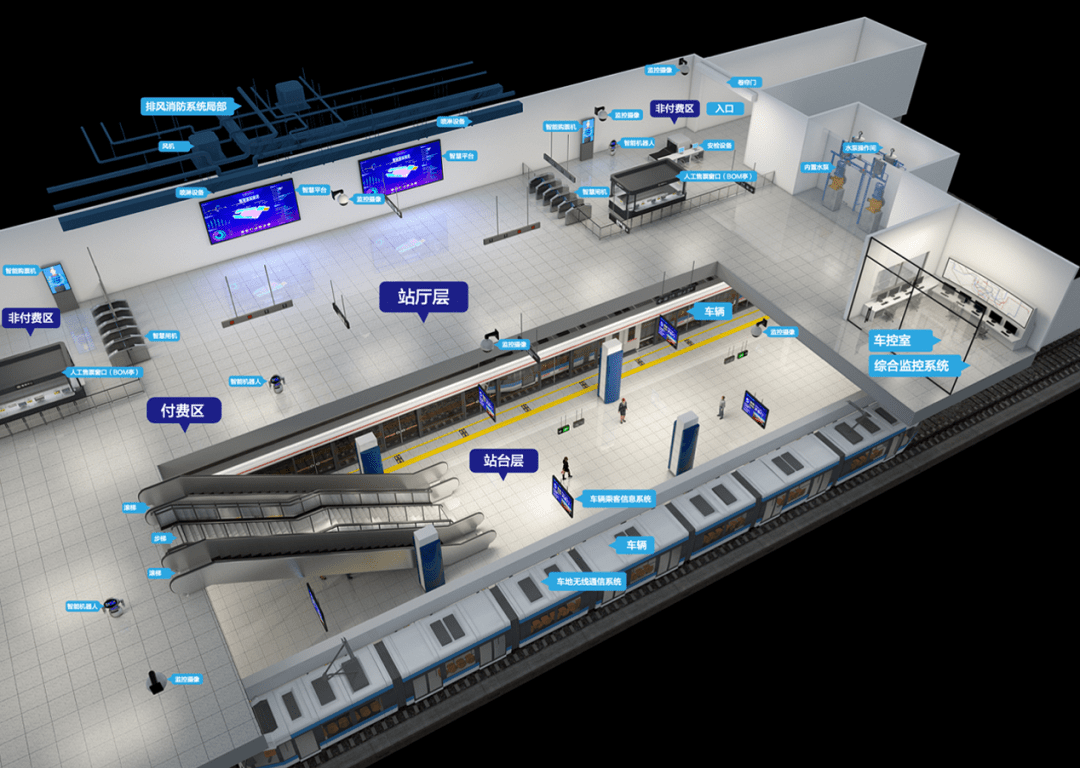
\includegraphics[width=0.8\textwidth]{车站示意图.png}
	\caption{车站示意图}
	\label{车站示意图}
\end{figure}

\begin{table}[h]
	\caption{与BAS接口的说明}
	\label{tab:与BAS接口的说明}
	\begin{tabular}{|l|l|l|l|l|l|}
		\hline
		FAS & \begin{tabular}[c]{@{}l@{}}BAS与\\ FAS的\\ 接口\end{tabular} & 车站 & \begin{tabular}[c]{@{}l@{}}车站控制室火灾\\ 报警控制器的端\\ 子排\end{tabular} & \begin{tabular}[c]{@{}l@{}}数据\\ 通信\\ 接口\end{tabular} & \begin{tabular}[c]{@{}l@{}}BAS按接收到的PLC模式指令,\\ 将所监控的设备转换成预定的\\ 火灾模式状态,并将其接收确\\ 认信号反馈给FAS系统\end{tabular} \\ \hline
	\end{tabular}
\end{table}

\section{FAS系统监控位置}
车站 CCTV 火警联动 FAS 功能:当车站的火警系统(FAS)触发火警报警后,车站的信息监控和控制系统(ISCS)会根据火警的位置信息,如果该区域设有监控摄像头,ISCS将自动检索相关摄像头的图像信息。车站的值班员可以通过鼠标控制位于火警现场的摄像头进行调整,而图像信息将通过FAS系统专门设置的监视器进行显示。

监控类表包括各种监测点的详细信息,例如监测点的位置、连接的设备和其他相关信息。这些监控点表的内容会因具体需求而不同,但样本表格通常包括监测点的各项属性和信息。

\section{具体设备选型}
综合以上讨论,给出具体的设备选型,以及安装位置如下表所示:

% Please add the following required packages to your document preamble:
% \usepackage{longtable}
% Note: It may be necessary to compile the document several times to get a multi-page table to line up properly
\begin{longtable}[c]{|l|l|l|l|}
	\caption{具体设备选型}
	\label{tab:my-table}\\
	\hline
	\multicolumn{1}{|c|}{\textbf{设备类型}} &
	\multicolumn{1}{c|}{\textbf{规格/型号}} &
	\multicolumn{1}{c|}{\textbf{功能描述}} &
	\multicolumn{1}{c|}{\textbf{部署位置}} \\ \hline
	\endfirsthead
	%
	\endhead
	%
	烟雾探测器   & Model XYZ123  & \begin{tabular}[c]{@{}l@{}}用于检测火灾\\ 产生的烟雾\end{tabular} & 站台、候车室、商业区  \\ \hline
	热感应器    & Model THM456  & \begin{tabular}[c]{@{}l@{}}检测异常温度\\ 升高\end{tabular}    & 电气设备区、闭合空间  \\ \hline
	一氧化碳检测器 & Model CO789   & \begin{tabular}[c]{@{}l@{}}检测一氧化碳\\ 水平\end{tabular}    & 地下通道、停车场    \\ \hline
	手动报警按钮  & Model MAN001  & \begin{tabular}[c]{@{}l@{}}用户手动激活\\ 火灾警报\end{tabular}  & 出入口、紧急出口旁   \\ \hline
	消防水泵    & Model PMP234  & 灭火用水泵                                                  & 消防水泵房       \\ \hline
	喷淋系统    & Model SPRY567 & \begin{tabular}[c]{@{}l@{}}自动喷水灭火\\ 系统\end{tabular}    & 整个车站覆盖区域    \\ \hline
	气体灭火系统  & Model GAS890  & \begin{tabular}[c]{@{}l@{}}在特定区域使\\ 用气体灭火\end{tabular} & 电气控制室、重要设备区 \\ \hline
	火灾警报器   & Model ALM101  & \begin{tabular}[c]{@{}l@{}}发出火灾警告\\ 声和光\end{tabular}   & 车站所有主要区域    \\ \hline
	紧急广播系统  & Model PA345   & \begin{tabular}[c]{@{}l@{}}紧急情况下的\\ 广播通知\end{tabular}  & 车站大厅、站台     \\ \hline
	紧急照明系统  & Model EML678  & \begin{tabular}[c]{@{}l@{}}火灾时提供照\\ 明引导疏散\end{tabular} & 走廊、出入口、紧急出口 \\ \hline
	安全疏散指示牌 & Model SIG901  & \begin{tabular}[c]{@{}l@{}}指示疏散路径\\ 和出口\end{tabular}   & 关键路径点、转角处   \\ \hline
	防烟排烟系统  & Model SMO234  & \begin{tabular}[c]{@{}l@{}}火灾时排除烟\\ 雾\end{tabular}     & 站台、商业区、候车室  \\ \hline
	紧急切断阀 &
	Model CUT456 &
	\begin{tabular}[c]{@{}l@{}}紧急情况下切\\ 断气体/水流\end{tabular} &
	\begin{tabular}[c]{@{}l@{}}主管道接入点、关键设\\ 备接入点\end{tabular} \\ \hline
	电源监控系统 &
	Model PWR789 &
	\begin{tabular}[c]{@{}l@{}}监控电源状态\\ ,保证紧急电\\ 源运行\end{tabular} &
	电气控制室、主配电室 \\ \hline
	防火门     & Model FDO012  & 防止火势蔓延                                                 & 紧急出口、关键分隔区域 \\ \hline
	紧急电源    & Model EPS345  & \begin{tabular}[c]{@{}l@{}}火灾时提供备\\ 用电源\end{tabular}   & 控制室、关键设备区   \\ \hline
\end{longtable}

\section{四遥点表设计}

四遥概述:四遥点表是一个用于记录和管理四遥(遥测、遥信、遥控、遥信控制)点的表格或数据库,通常用于监测和控制远程设备或系统。四遥点表列出了各种遥测、遥信、遥控和遥信控制点的详细信息,包括点的名称、点的描述、点的类型、点的状态以及其他相关信息。

这些表格通常由工程师和运维人员使用,以便了解远程设备和系统的状态,进行实时监测、故障排除和远程控制。四遥点表有助于提高运营效率、确保系统的可靠性,并快速应对潜在的问题和紧急情况。

四遥点表的具体格式和内容会根据应用领域和系统的不同而有所变化,但通常包括了点的基本信息,如点名称、点描述、点类型(遥测、遥信、遥控、遥信控制)、点的状态以及其他用于标识和管理遥点的字段。

四遥系统是指遥测、遥信、遥控和遥调功能系统。以下是这些功能的详细描述:

\begin{itemize}
	\item \textbf{遥测(遥测信息)}:这是一种远程测量功能,用于采集并传送运行参数。它包括各种电气量,如线路上的电压、电流、功率等模拟量(AI),以及负荷潮流等信息。
	
	\item \textbf{遥信(遥信信息)}:遥信功能用于远程信号传输,采集并传送各种保护和开关量信息(DI)。
	
	\item \textbf{遥控(遥控信息)}:这是一项远程控制功能,用于接受并执行遥控命令。主要应用于分合闸等操作,以对远程的一些开关控制设备进行远程控制(DO)。
	
	\item \textbf{遥调(遥调信息)}:遥调功能用于远程调节,接受并执行遥调命令。它主要用于对远程的控制量设备进行远程调试,例如调整发电机的输出功率(AO)。
\end{itemize}

四遥系统在电力和自动化控制领域具有广泛的应用,它能够实现远程监测、信号传输、控制和调节等功能,提高了系统的运行效率和可靠性。

四遥点表

通过前文对车站机电设备监控点的分析,根据IEC60870-5-101规约得到如下的四遥点表。

其中FAS系统遥信的点表如下:
% Please add the following required packages to your document preamble:
% \usepackage{longtable}
% Note: It may be necessary to compile the document several times to get a multi-page table to line up properly
\begin{longtable}[c]{|l|l|l|l|l|}
	\caption{FAS遥信}
	\label{tab:my-table}\\
	\hline
	\textbf{序号} & \textbf{信号体地址} & \textbf{信号点名称} & \textbf{状态} & \textbf{备注} \\ \hline
	\endfirsthead
	%
	\endhead
	%
	1           & 1H             & 一层烟雾报警1状态      & 正常/报警       &             \\ \hline
	2           & 2H             & 二层烟雾报警2状态      & 正常/报警       &             \\ \hline
	3           & 3H             & 三层烟雾报警3状态      & 正常/报警       &             \\ \hline
	4           & 4H             & 四层烟雾报警4状态      & 正常/报警       &             \\ \hline
	5           & 5H             & 一层手动报警1激活状态    & 未激活/激活      &             \\ \hline
	6           & 6H             & 二层手动报警2激活状态    & 未激活/激活      &             \\ \hline
	7           & 7H             & 三层手动报警3激活状态    & 未激活/激活      &             \\ \hline
	8           & 8H             & 四层手动报警4激活状态    & 未激活/激活      &             \\ \hline
	9           & 9H             & 一层喷淋系统1状态      & 关闭/开启       &             \\ \hline
	10          & AH             & 二层喷淋系统2状态      & 关闭/开启       &             \\ \hline
	11          & BH             & 三层喷淋系统3状态      & 关闭/开启       &             \\ \hline
	12          & CH             & 四层喷淋系统4状态      & 关闭/开启       &             \\ \hline
	13          & DH             & 一层防火门1关闭状态     & 打开/关闭       &             \\ \hline
	14          & EH             & 二层防火门2关闭状态     & 打开/关闭       &             \\ \hline
	15          & FH             & 三层防火门3关闭状态     & 打开/关闭       &             \\ \hline
	16          & 10H            & 四层防火门4关闭状态     & 打开/关闭       &             \\ \hline
	17          & 11H            & 一层紧急照明1系统状态    & 未激活/激活      &             \\ \hline
	18          & 12H            & 二层紧急照明2系统状态    & 未激活/激活      &             \\ \hline
	19          & 13H            & 三层紧急照明3系统状态    & 未激活/激活      &             \\ \hline
	20          & 14H            & 四层紧急照明4系统状态    & 未激活/激活      &             \\ \hline
	21          & 15H            & 地下室燃气泄漏监测      & 正常/泄漏       &             \\ \hline
	22          & 16H            & 一层空气质量指标       & 良好/污染       &             \\ \hline
	23          & 17H            & 二层空气质量指标       & 良好/污染       &             \\ \hline
	24          & 18H            & 三层空气质量指标       & 良好/污染       &             \\ \hline
	25          & 19H            & 四层空气质量指标       & 良好/污染       &             \\ \hline
\end{longtable}

其中FAS系统遥测的点表如下:

% Please add the following required packages to your document preamble:
% \usepackage{longtable}
% Note: It may be necessary to compile the document several times to get a multi-page table to line up properly
\begin{longtable}[c]{|l|l|l|l|l|}
	\caption{FAS遥测}
	\label{tab:my-table}\\
	\hline
	\textbf{序号} & \textbf{信号体地址} & \textbf{信号点名称} & \textbf{单位} & \textbf{备注} \\ \hline
	\endfirsthead
	%
	\endhead
	%
	1           & 4001H          & 一层温湿度监测点1温度    & °C          &             \\ \hline
	2           & 4002H          & 一层温湿度监测点2温度    & °C          &             \\ \hline
	3           & 4003H          & 一层温湿度监测点3温度    & °C          &             \\ \hline
	4           & 4004H          & 二层温湿度监测点1温度    & °C          &             \\ \hline
	5           & 4005H          & 二层温湿度监测点2温度    & °C          &             \\ \hline
	6           & 4006H          & 二层温湿度监测点3温度    & °C          &             \\ \hline
	7           & 4007H          & 三层温湿度监测点1温度    & °C          &             \\ \hline
	8           & 4008H          & 三层温湿度监测点2温度    & °C          &             \\ \hline
	9           & 4009H          & 三层温湿度监测点3温度    & °C          &             \\ \hline
	10          & 400AH          & 四层温湿度监测点1温度    & °C          &             \\ \hline
	11          & 400BH          & 四层温湿度监测点2温度    & °C          &             \\ \hline
	12          & 400CH          & 四层温湿度监测点3温度    & Ppm         &             \\ \hline
	13          & 400DH          & 一层温湿度监测点1湿度    & Ppm         &             \\ \hline
	14          & 400EH          & 一层温湿度监测点2湿度    & Ppm         &             \\ \hline
	15          & 400FH          & 一层温湿度监测点3湿度    & Ppm         &             \\ \hline
	16          & 4010H          & 二层温湿度监测点1湿度    & Ppm         &             \\ \hline
	17          & 4011H          & 二层温湿度监测点2湿度    & Ppm         &             \\ \hline
	18          & 4012H          & 二层温湿度监测点3湿度    & Ppm         &             \\ \hline
	19          & 4013H          & 气温差监测点1        & °C          &             \\ \hline
	20          & 4014H          & 气温差监测点2        & °C          &             \\ \hline
	21          & 4013H          & 水池水位1          & cm          &             \\ \hline
	22          & 4014H          & 水池水位2          & cm          &             \\ \hline
	23          & 4015H          & 供水总管供水温度       & °C          &             \\ \hline
	24          & 4016H          & 供水总管水管压差       & Pa          &             \\ \hline
	25          & 4017H          & 地灾气体(水)流速      & L/min       &             \\ \hline
	26          & 4018H          & 卷帘门1门磁信号       & ——          & 4           \\ \hline
	27          & 4019H          & 卷帘门2门磁信号       & ——          & 4           \\ \hline
\end{longtable}

值得注意的是,通常FAS系统中不常见,但可能包括设置警报器的敏感度等。
其中FAS系统遥控的点表如下:

% Please add the following required packages to your document preamble:
% \usepackage{longtable}
% Note: It may be necessary to compile the document several times to get a multi-page table to line up properly
\begin{longtable}[c]{|l|l|l|l|l|}
	\caption{FAS遥控}
	\label{tab:my-table}\\
	\hline
	\textbf{序号} & \textbf{信号体地址} & \textbf{信号点名称} & \textbf{单位} & \textbf{备注} \\ \hline
	\endfirsthead
	%
	\endhead
	%
	1           & 6001H          & 一层烟雾报警器1启停     & ——          &             \\ \hline
	2           & 6002H          & 一层烟雾报警器2启停     & ——          &             \\ \hline
	3           & 6003H          & 一层烟雾报警器3启停     & ——          &             \\ \hline
	4           & 6004H          & 二层烟雾报警器1启停     & ——          &             \\ \hline
	5           & 6005H          & 二层烟雾报警器2启停     & ——          &             \\ \hline
	6           & 6006H          & 二层烟雾报警器3启停     & ——          &             \\ \hline
	7           & 6007H          & 三层烟雾报警器1启停     & ——          &             \\ \hline
	8           & 6008H          & 三层烟雾报警器2启停     & ——          &             \\ \hline
	9           & 6009H          & 三层烟雾报警器3启停     & ——          &             \\ \hline
	10          & 600AH          & 一层防火门控制系统1     & ——          &             \\ \hline
	11          & 600BH          & 二层防火门控制系统2     & ——          &             \\ \hline
	12          & 600CH          & 一层紧急电源切换       & ——          &             \\ \hline
	13          & 600DH          & 车站电梯紧急控制       & ——          &             \\ \hline
	14          & 600EH          & 逃生指示系统启停       & ——          &             \\ \hline
	15          & 600FH          & 车站通风系统控制       & ——          &             \\ \hline
	16          & 6010H          & 安全监控系统启停       & ——          &             \\ \hline
	17          & 6011H          & 人员疏散指令         & ——          &             \\ \hline
	18          & 6012H          & 水泵控制           & ——          &             \\ \hline
	19          & 6013H          & 燃气阀门紧急关闭       & ——          &             \\ \hline
	20          & 6014H          & 紧急停车指令         & ——          &             \\ \hline
\end{longtable}

其中FAS系统遥调的点表如下:
% Please add the following required packages to your document preamble:
% \usepackage{longtable}
% Note: It may be necessary to compile the document several times to get a multi-page table to line up properly
\begin{longtable}[c]{|l|l|l|l|l|}
	\caption{FAS遥调}
	\label{tab:my-table}\\
	\hline
	\textbf{序号} & \textbf{信号体地址} & \textbf{信号点名称} & \textbf{单位} & \textbf{备注} \\ \hline
	\endfirsthead
	%
	\endhead
	%
	1           & 6201H          & 一层照明亮度调节       & \%          &             \\ \hline
	2           & 6202H          & 二层照明亮度调节       & \%          &             \\ \hline
	3           & 6203H          & 三层照明亮度调节       & \%          &             \\ \hline
	4           & 6204H          & 四层照明亮度调节       & \%          &             \\ \hline
	5           & 6205H          & 一层空调温度设定       & °C          &             \\ \hline
	6           & 6206H          & 二层空调温度设定       & °C          &             \\ \hline
	7           & 6207H          & 三层空调温度设定       & °C          &             \\ \hline
	8           & 6208H          & 四层空调温度设定       & °C          &             \\ \hline
	9           & 6209H          & 一层通风系统流量调节     & m³/min      &             \\ \hline
	10          & 620AH          & 二层通风系统流量调节     & m³/min      &             \\ \hline
	11          & 620BH          & 三层通风系统流量调节     & m³/min      &             \\ \hline
	12          & 620CH          & 四层通风系统流量调节     & m³/min      &             \\ \hline
	13          & 620DH          & 一层喷淋系统压力调节     & bar         &             \\ \hline
	14          & 620EH          & 二层喷淋系统压力调节     & bar         &             \\ \hline
	15          & 620FH          & 三层喷淋系统压力调节     & bar         &             \\ \hline
	16          & 6210H          & 四层喷淋系统压力调节     & bar         &             \\ \hline
	17          & 6211H          & 全站紧急广播音量调节     & dB          &             \\ \hline
	18          & 6212H          & 一层CO2浓度报警阈值设定  & ppm         &             \\ \hline
	19          & 6213H          & 二层CO2浓度报警阈值设定  & ppm         &             \\ \hline
	20          & 6214H          & 三层CO2浓度报警阈值设定  & ppm         &             \\ \hline
	21          & 6215H          & 四层CO2浓度报警阈值设定  & ppm         &             \\ \hline
\end{longtable}